\chapter{Star Trackers}

Existem várias formas de se medir a atitude, porém, a forma mais amplamente utilizada em satélites profissionais de grande porte são os seguidores de estrelas (start trackers). A tecnologia de tais sistemas vêm evoluindo nos últimos anos, com a rápida melhoria dos sensores CCD (charge-coupled device), e tecnologias de análise de imagem. Porém,  erros são  inerentes a qualquer medida, por mais pequeno que um erro possa ser, pode levar a uma identificação errônea de uma estrela, resultado em um erro completo de posicionamento.

Star Trackers funcionam capturando imagens de estrelas e comparando a tabelas salvas em memória ~\cite[]{Diaz}. Desta forma, o satélite é capaz de identificar a sua atitude.

No entanto, os sistemas comerciais possuem preço elevado, consumo de energia elevado e massa elevada para pequenos satélites, como é mostrado na figura ~\ref{fig:Comp_star_trackers_comerciais}.

\begin{figure}[!h]
	\centering
	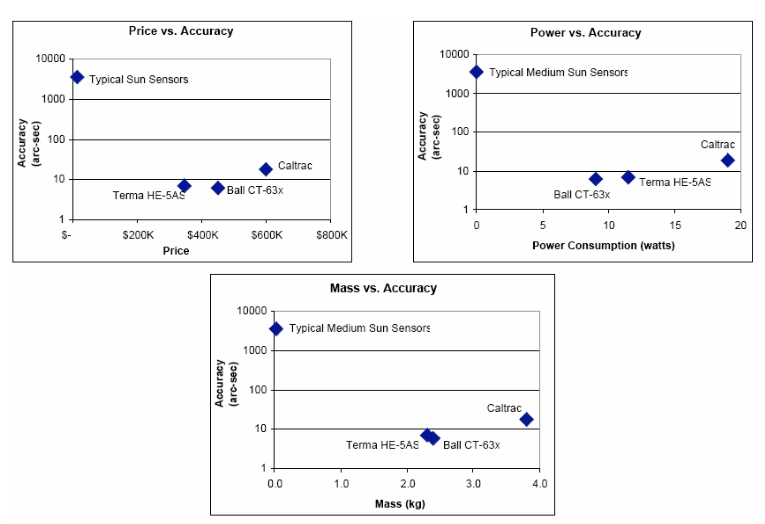
\includegraphics[width=.7\columnwidth]{images/comp_star_trackers.png}
	\caption{Comparação de Star Trackers comerciais. (a) Relação entre preço e precisão, (b) Relação entre energia consumida e precisão, (c) Relação entre massa e precisão. Fonte: ~\cite[]{Diaz}}
	\label{fig:Comp_star_trackers_comerciais}
\end{figure}

\section{Etapas de operação}


As etapas de operação desse sistema costumam seguir a estrutura apresentada na Figura ~\ref{fig:etapas_star_trackers}.


\begin{figure}[!h]
	\centering
	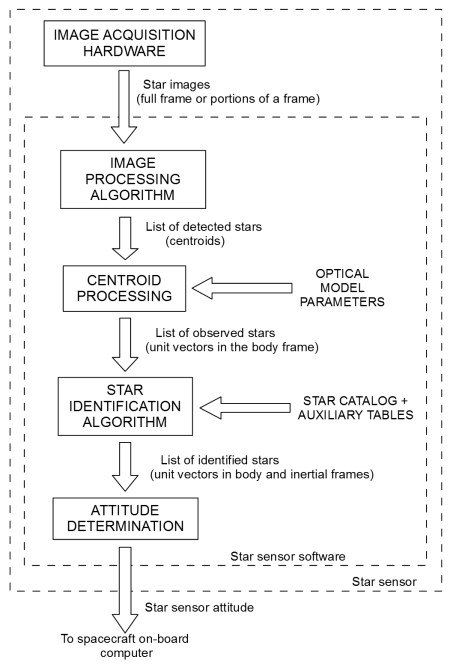
\includegraphics[width=.7\columnwidth]{images/etapas.jpg}
	\caption{Etapas de funcionamento de um star tracker. Fonte: ~\cite[]{Fialho}}
	\label{fig:etapas_star_trackers}
\end{figure}

A primeira etapa de operação, consiste  na aquisição da imagem a ser utilizada, para tal é utilizado um CCD acoplado a um conjunto de lentes. A escolha desse componentes deve levar em conta uma série de parâmetros, tais como: abertura do campo visual, precisão, volume, peso e outros a variar com a  missão do cubesat ~\cite[]{Carvalho}. Neste projeto a aquisição de imagens será feita com uma webcam.

O algoritmo de processamento juntamente com processamento de centróide, são responsáveis por localizar cada uma das estrelas e determinar sua localização e intensidade.

O algoritmo de identificação de estrelas é responsável por fazer a relação entre as estrelas identificadas na observação e as estrelas contidas no banco de dados. A identificação de uma estrela envolve a análise das relações entre as diversas estrelas observadas, para tal utiliza-se algoritmos como de  Planar Triangles ~\cite[]{Cole}.

Por fim, é determinada a atitude do cubesat, que pode ser feita utilizando ângulos de Euler ou quaternions.

Para realizar testes no sistema,  será implementado um simulador estrelar, seguindo o método demonstrado por Tappe ~\cite[]{Tappe}. Por fim, serão realizados testes com imagens reais obtidas por webcams  ou câmeras de celulares.

\section{Esfera celeste}

Para aplicação no rastreador estelar, as estrelas são representadas através de uma esfera celeste, na  qual as estrelas são distribuídas em uma esfera ao redor do centro, que na aplicação de satélites é a própria Terra. Devido a diferença de escalas da distância das estrelas a Terra e o tamanho da Terra , pode-se considerar que qualquer ponto na Terra e na órbita terrestre, estão exatamente no centro da esfera. O erro gerado por tal simplificação só  se tornaria visível em missões em que o veículo espacial se retirasse do sistema solar, o que não é caso para Cubesats atuais.

Também é completamente desprezado qualquer movimento que os astros tenham em relação uns aos outros, pois estes movimentos são praticamente nulos em nossas análises.

Isto se deve o fato de que, o quanto maior for a distância do observador a um objeto, menor será a variação angular para um mesmo movimento linear do objeto, como por exemplo pode-se observar que aviões aparentam estar extremamente lento para um observador na Terra, No caso do sistema estrelar, esse efeito é ainda maior, permitindo desprezar esse movimento relativo entre as estrelas sem nenhum prejuízo prático a precisão ~\cite[]{Carvalho}.

Nesta abordagem, algumas das características da Terra são representadas na esfera, como o eixo de rotação em torno de si mesma (rotação) e os pólos geográficos, que são nomeados respectivamente eixo e pólos celestes. Com isto facilita-se a localização dos astro na esfera. Para isto cria-se circunferências envolvendo a esfera, concorrendo nos polos (meridianos), com circunferências perpendiculares ao eixo de rotação(paralelos) ~\cite[]{Carvalho}.

\begin{figure}[!h]
	\centering
	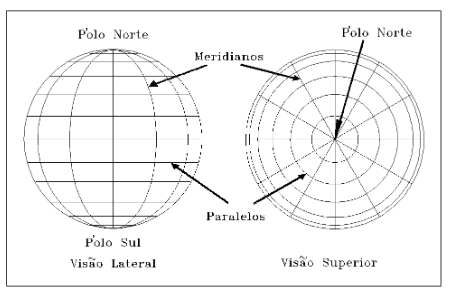
\includegraphics[width=.7\columnwidth]{images/codficacao_cod_esferas_celetes.png}
	\caption{Codificação de coordenadas na esfera celeste. Fonte: ~\cite[]{Carvalho}}
	\label{fig:codficacao_cod_esferas_celetes}
\end{figure}

Como referência tem-se o paralelo central, conhecido como paralelo do Equador,  o meridiano de referência é o que contém o ponto vernal . O ponto vernal é o momento em que o Sol passa o Equador de Sul para Norte, isto ocorre pois a rotação da Terra em torno do próprio eixo está inclinada em relação ao plano da trajetória elíptica da Terra em torno do Sol.Como é visto na Figura  ~\ref{fig:inclinacao}.

\begin{figure}[!h]
	\centering
	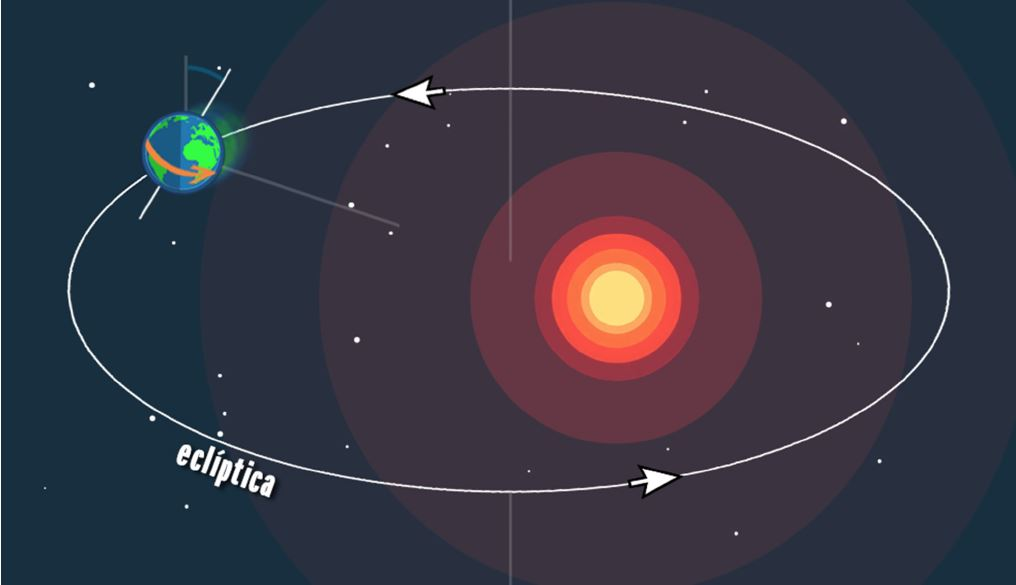
\includegraphics[width=.7\columnwidth]{images/inclinacao.jpg}
	\caption{Inclinação órbita terrestre. Fonte: ~\cite[]{Portal_do_Astronomo}}
	\label{fig:inclinacao}
\end{figure}

\section{Referencial Inercial Terrestre}

Utilizando os conceito da  Esfera celeste, cria-se o referencial inercial terrestres, em que o eixo x está alinhado com vetor radial partindo do Sol em direção a Terra no (linha de Áries), que é o equinócio de inverno, o eixo z é alinhado com o eixo de rotação da Terra, e o eixo y segue a regra da mão direita, conforme as figuras ~\ref{fig:Frame_inercial_terrestre} e ~\ref{fig:Referencial_inercial}.

\begin{figure}[!h]
	\centering
	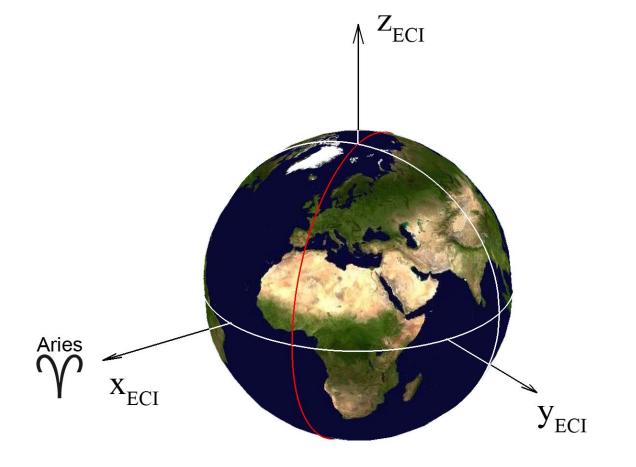
\includegraphics[width=.7\columnwidth]{images/Frame_inercial_terrestre.png}
	\caption{Frame inercial terrestre. Fonte: ~\cite[]{Diaz}}
	\label{fig:Frame_inercial_terrestre}
\end{figure}

\begin{figure}[!h]
	\centering
	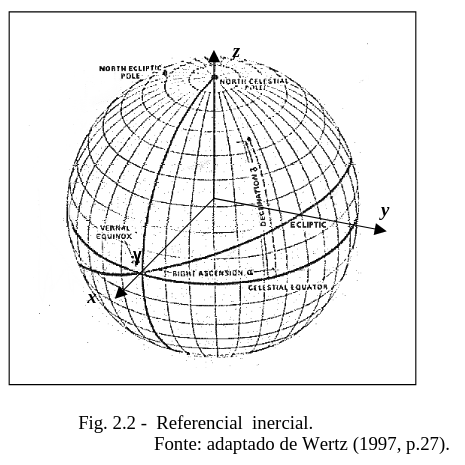
\includegraphics[width=.7\columnwidth]{images/Referencial_inercial.png}
	\caption{Referencial inercial. Fonte: ~\cite[]{Carvalho}}
	\label{fig:Referencial_inercial}
\end{figure}

As estrelas são catalogadas utilizando os pontos de referência, utilizando-se de um sistema de coordenadas polares, com duas coordenadas angulares. Um dos ângulos é definido a partir dos meridianos, que é a ascensão reta , o ponto de ares é o marco zero, a ascensão da reta varia de 0 a 360 graus.

A outra coordenada polar é a declinação $\gamma$, que é o ângulo entre a estrela e o paralelo do equador, variando de -90 a 90 graus. A Figura ~\ref{fig:Sistema_de_coordenadas_vetorial} mostra sua representação.

\begin{figure}[!h]
	\centering
	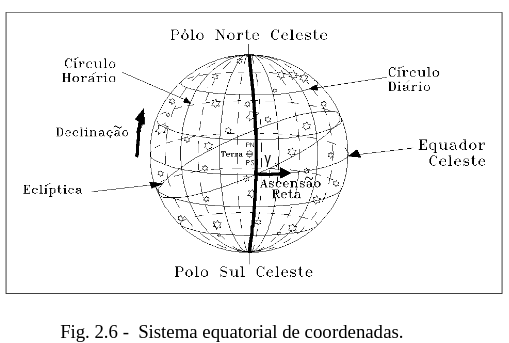
\includegraphics[width=.7\columnwidth]{images/Sistema_equatorial_de_coordenadas.png}
	\caption{Sistema equatorial de coordenadas. Fonte: ~\cite[]{Carvalho}}
	\label{fig:Sistema_equatorial_de_coordenadas}
\end{figure}

A transformação do sistema de coordenadas polares para coordenadas cartesianas é feita  com base na Figura 9.

\begin{figure}[!h]
	\centering
	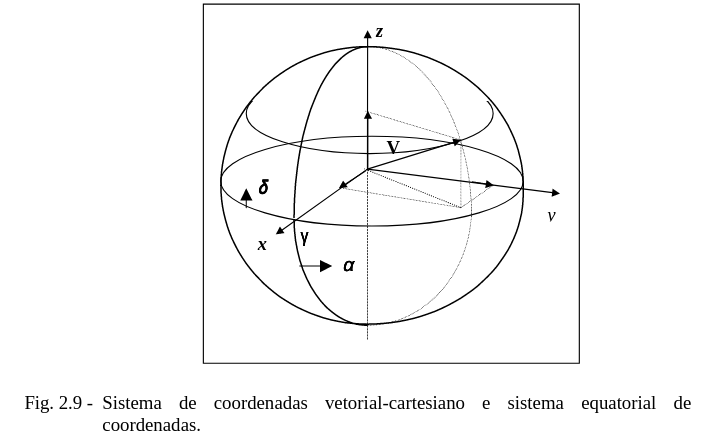
\includegraphics[width=.7\columnwidth]{images/Sistema_de_coordenadas_vetorial.png}
	\caption{Sistema de coordenadas vetorial- cartesiano e sistema equatorial de coordenadas. Fonte: ~\cite[]{Carvalho}}
	\label{fig:Sistema_de_coordenadas_vetorial}
\end{figure}


Todas as estrelas catalogadas são descritas na superfície de uma esfera unitária  com centro cociente a terra, portanto, o módulo do vetor que sai do centro da esfera até a estrela é sempre 1.
\begin{equation}
	\left| \overrightarrow{V}\right|=1,
	\label{eq:1}
\end{equation}
Dessa forma desconsidera-se o valor do raio nas equações  de  transformação de coordenadas, a elaboração das equações é realizada através da análise das relações trigonométricas do sistemas, o que resulta em:

\begin{equation}
	V_{x}=cos(\gamma)cos(\alpha),
	\label{eq:2}
\end{equation}

\begin{equation}
	V_{y}=cos(\gamma)sin(\alpha),
	\label{eq:3}
\end{equation}

\begin{equation}
	V_{z}=sin(\gamma),
	\label{eq:4}
\end{equation}

\section{Referencial do cubesat}

O referencial do cubesat é alinhado geometricamente com o equipamento, dessa forma ele representa a posição do cubesat em si. Como pode ser visto na figura ~\ref{fig:Referencia_do_Cubesat}.

\begin{figure}[!h]
	\centering
	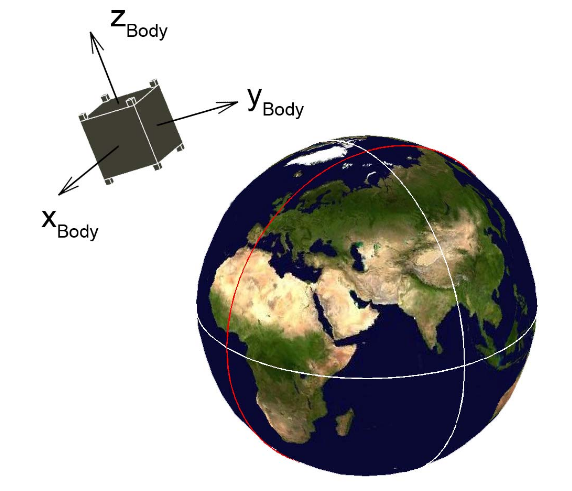
\includegraphics[width=.7\columnwidth]{images/Referencia_do_Cubesat.png}
	\caption{Referência do Cubesat. Fonte: ~\cite[]{Diaz}}
	\label{fig:Referencia_do_Cubesat}
\end{figure}

O referencial da câmera, tem os eixos x e y normal ao plano da imagem, a imagem captada pela câmera se encontra a uma distância unitária do cubesat no eixo Z, o motivo de se utilizar uma distância unitária e demais informações sobre o frame de câmera , serão tratados no capítulo de projeções em perspectiva. Neste trabalho é considerado que o referencial do cubesat é o mesmo da câmera, como é visto na figura ~\ref{fig:Camera_Frame}.

\begin{figure}[h]
	\centering
	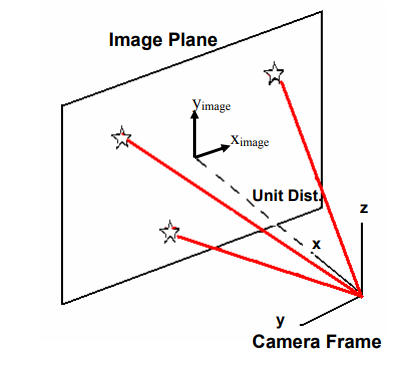
\includegraphics[width=.7\columnwidth]{images/Camera_Frame.png}
	\caption{Camera Frame. Fonte: ~\cite[]{Diaz}}
	\label{fig:Camera_Frame}
\end{figure}

\section{Catalogo}

A criação do catálogo é realizada por satélites especialmente criados e lançados com este propósito, como o é o caso do NASA I/239, que compõem o banco de dados do Hipparcos and Tycho. Este banco de dados é encontrado em ~\cite[]{ESA}.

O banco de dados possui uma tabela principal de informações, com o formato mostrado na figura ~\ref{fig:Resumo_impetracao_parte_esquerda_Hipparcos}.

\begin{figure}[h]
	\centering
	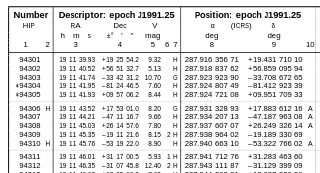
\includegraphics[width=.7\columnwidth]{images/Resumo_impetracao_parte_esquerda_Hipparcos.png}
	\caption{Resumo de impetração da parte esquerda do catálogo Hipparcos. Fonte: ~\cite[]{ESA}}
	\label{fig:Resumo_impetracao_parte_esquerda_Hipparcos}
\end{figure}

Essa tabela possui muitas informações que não serão utilizadas, incluindo uma quantidade de estrela muito grande, portanto o banco de dados foi filtrado com apenas alguns campos de dados restantes, o que mostrado na figura ~\ref{fig:Caracteristicas_matriz}.

\begin{figure}[h]
	\centering
	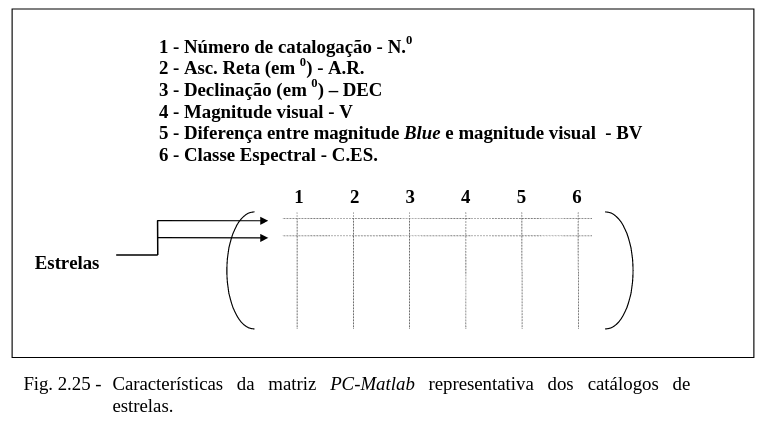
\includegraphics[width=.7\columnwidth]{images/Caracteristicas_matriz.png}
	\caption{Características de matriz representativa do catálogo estelar. Fonte: ~\cite[]{Carvalho}}
	\label{fig:Caracteristicas_matriz}
\end{figure}

O banco de dados estelar é filtrado por colunas, gerando um catálogo com as informações mostradas na Figura 12. Além disto  se realiza uma filtragem por estrelas com magnitude quatro ou inferior, o que significa que apenas as estrelas mais brilhantes permaneceram na base de dados do sistema. Para a visualização das estrelas restantes utiliza-se o sistema equatorial de coordenadas, com isto os plots das figuras ~\ref{fig:Rrepresentacao_2D} e \ref{fig:Representacao_3D} podem ser realizados.

\begin{figure}[h]
	\centering
	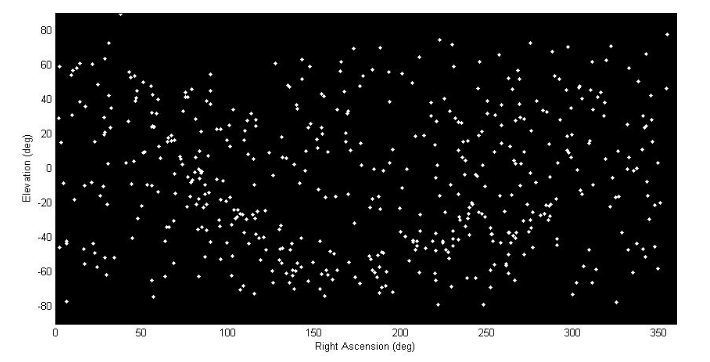
\includegraphics[width=.7\columnwidth]{images/Rrepresentacao_2D.png}
	\caption{Catálogo estelar representação em 2D. Fonte: ~\cite[]{Diaz}}
	\label{fig:Rrepresentacao_2D}
\end{figure}

\begin{figure}[h]
	\centering
	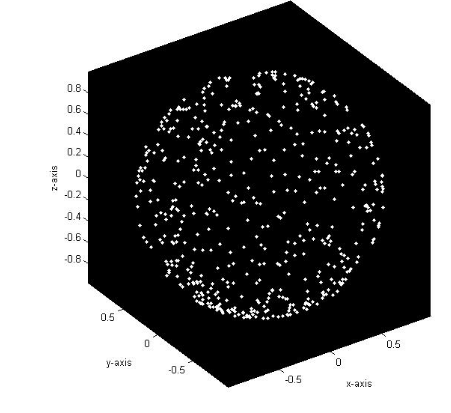
\includegraphics[width=.7\columnwidth]{images/Representacao_3D.png}
	\caption{Catálogo estelar representação em 3D. Fonte: ~\cite[]{Diaz}}
	\label{fig:Representacao_3D}
\end{figure}

\section{Análise de imagem}

Analise de imagem é o primeiro passo na analise de dados de nosso sistema, no caso a analise deve ter a capacidade de localizar a posição correta das estrelas presentes no campo de visão da camera.
Erros nesta atapa da analise pode fazer o resonhecimento da posição angular do sateleite se tornar impossivel.

\subsection{Distorções em imagens}
As correções de distorções nas imagens captadas devem ser realizadas, com os erros não podendo ser ignorados, pois a distorção de imagem pode causar erros na localização das estrelas. Estas distorções se dividem em dois componentes predomintantes, uma sendo a radial e outra tangencial.
Além disto, existem distorções de contrução das lentes, distorções de desalinhamento da lente em relação ao centro da Matriz CCD da câmera.

\subsubsection{Distorção radial}
Distorção radial é vista quando utiza-se câmera com grandes ângulos e com pequena distância focal~\cite[]{Mallon}.
Os efeitos da distorção radial são representados na figura ~\ref{fig:Distorcao_radial}.

\begin{figure}[h]
	\centering
	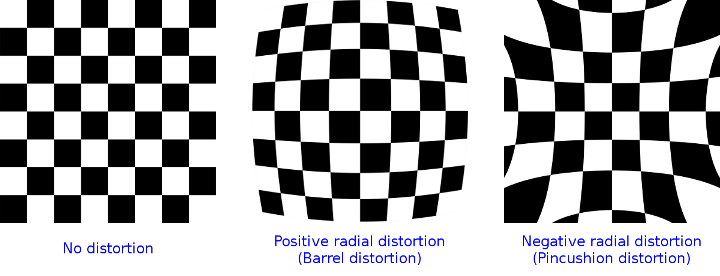
\includegraphics[width=.7\columnwidth]{images/Distorcao_radial.png}
	\caption{Distorção radial. Fonte: ~\cite[]{ozcakir_2020}}
	\label{fig:Distorcao_radial}
\end{figure}

Esta distorção pode ser corrigida através de diferentes métodos, neste trabalho utiliza-se o método matemático descrito pelo ~\cite[]{opencv_library}.
Dessa forma a distorção radial é corrigida através das equações ~\ref{eq:Distorcao_radial_x} e ~\ref{eq:Distorcao_radial_y}.

\begin{equation}
	X_{corrigido} = X_{original} (1 + k_1 r^2 + k_2 r^4 + k_3 r^6)
	\label{eq:Distorcao_radial_x}
\end{equation}

\begin{equation}
	Y_{corrigido} = Y_{original} (1 + k_1 r^2 + k_2 r^4 + k_3 r^6)
	\label{eq:Distorcao_radial_y}
\end{equation}

\subsubsection{Distorção tangencial}
Distorçoes Tangencial ocorrem quando a câmera e o plano da imagem não estão em paralelo ~\cite[]{ozcakir_2020}.
Os efeitos da distorção tangencial são representados na figura ~\ref{fig:Distorcao_tangencial}.

\begin{figure}[h]
	\centering
	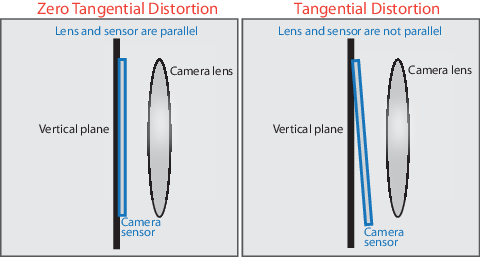
\includegraphics[width=.7\columnwidth]{images/Distorcao_tangencial.png}
	\caption{Distorção tangencial. Fonte: ~\cite[]{ozcakir_2020}}
	\label{fig:Distorcao_tangencial}
\end{figure}

Esta distorção é corrigida através das equações ~\ref{eq:Distorcao_tangencial_x} e ~\ref{eq:Distorcao_tangencial_y}.

\begin{equation}
	X_{corrigido} = X_{original} (1 + p_1 r^2 + p_2 r^4 + p_3 r^6)
	\label{eq:Distorcao_tangencial_x}
\end{equation}

\begin{equation}
	Y_{corrigido} = Y_{original} (1 + p_1 r^2 + p_2 r^4 + p_3 r^6)
	\label{eq:Distorcao_tangencial_y}
\end{equation}

Resalta-se que a ferramenta de simulação estrelar desenvolvida para este trabalho não possui distorcão tangencial, pois a câmera e o plano da imagem estão em paralelo.

\section{Detecção de estrelas}
\subsection{Localização de circulos}
Os métodos de detecção de círcurlos em geral consiste nas variações do método de Hough Transform(HT) ,como o standard Hough Transform, o Fast Hough Transform de de Li et al.

Para aplicar um método de Hough Transform, é necessario se aplicar um filtro para detecção de bordas na imagem, pois HT utiliza a posição destes pixels para calcular o possível centro do círculo.
Neste trabalho utiliza-se um filtro clássico de Canny, pois o ganho em qualidade de detecção de outros algorítmos de análise, como o de onda contínua, que utilizam recursos computacionais maiores, como é mostrado por Kobylin ~\cite[]{kobylin2014comparison}

HT faz utilização da equação do círculo, para fazer a detecção do círculo, o método consiste em se testar todas as possilidades de círculos possíveis para cada pixel na borda de cada ponto na imagem.
Uma vez feito todos os câlculos para cada um dos pixels de borda, o mêtodo seleciona o circulo com maior recorrência em diferentes pixels. Yuen demonstra sua aplicação em diferentes variações ~\cite[]{YUEN199071}.

\subsection{Transformação de coordenadas}
A localização das entrelas occore em coordenadas cartesianas em relação ao centro do Campo de visão da câmera, utilizando o referêncial já demonstrado, porém é mais conveniente que a localização seja representada através de coordenadas polares, para isso é necessário se realizar a transformação de coordenadas.
Seguindo as formulas  ~\ref{eq:transformacao_cordenadas_theta} e ~\ref{eq:transformacao_cordenadas_r}.

\begin{equation}
	\theta  = 
	\begin{cases}
		\arctan \left( \frac{y}{x} \right), & \text{se } x >= 0 \\
		\arctan \left( \frac{y}{x} \right) + \pi, & \text{se } x < 0 \\
	\end{cases}
	\label{eq:transformacao_cordenadas_theta}
\end{equation}

\begin{equation}
	r = \sqrt{x^2 + y^2}
	\label{eq:transformacao_cordenadas_r}
\end{equation}

A variável \textbf{r} é então transformada em uma variável ângular, através de uma relação linear. Com os coeficientes sendo calculados através de uma imagem de referência.

\begin{equation}
	r_{angular} = r * C_{converção}
	\label{eq:transformacao_cordenadas_theta_angular}
\end{equation}

\subsection{Cálculo do ângulos entre estrelas}
O calculo da distância entre as estrelas presentes no FOV é realizado através da fórmula ~\ref{eq:calculo_distancia_estrelas}.
Além disto, é aplicado um valor máximo para limitiar o ângulo entre as estrelas, pois isto diminui a utilização de recursos computacionais.

\begin{equation}
	dist_{angular} = \sqrt{r_{estrela_1}^2 + r_{estrela_2}^2 - 2 * r_{estrela_1} * r_{estrela_2} * cos(\theta_{estrela_1} - \theta_{estrela_2})}
	\label{eq:calculo_distancia_estrelas}
\end{equation}

\subsection{Cálculo da área antre estrelas}

A área entre o conjunto de 3 estrelas é calculada através da fórmula de Heron ~\ref{eq:calculo_area_estrelas}.
\begin{equation}
	area = \sqrt{p(p-a)(p-b)(p-c)}
	\label{eq:calculo_area_estrelas}
\end{equation}

Em que \textbf{p} é a metade do perímetro do triângulo, e \textbf{a}, \textbf{b} e \textbf{c} são as distâncias entre as estrelas.

\begin{equation}
	p = \frac{a+b+c}{2}
	\label{eq:calculo_area_estrelas_p}
\end{equation}

\subsection{Cálculo do momento entre estrelas}

O momento entre o conjunto de 3 estrelas é calculado através da fórmula ~\ref{eq:calculo_momento_estrelas}.

\begin{equation}
	momento = \frac{area (a^2 + b^2 + c^2)}{36}
	\label{eq:calculo_momento_estrelas}
\end{equation}

\section{Banco de dados}
Uma vez feito o reconhecimento dos ângulos, momentos e áreas da estrelas presentes no FOV, é necessário  comparar estas relações encontradas no imagem com as relações presentes no banco de dados.

Devido as limitações energéticas do sistema, é necessário que a estrutura do banco de dados seja otimizada para a resolução do problema em questão.
Assim como métodos de busca no banco de dados e refino de possibilidades possiveis, são implementados para agilizar a operação do sistema e diminuir o tamanho do banco de dados.

\subsection{Estrutura e pesquisa de dados }
O sistema possui duas fases distintas de operação, uma quando o sistema se encontra sem nenhuma posição prévia de confiança, outra é quando o sistema já esta em operação por uma tempo e portanto já consegue determinar a sua posição de forma mais rapida utilizado outros metodos de pesquisa.

\subsubsection{K vector}

O método \textbf{k vector} é desonlvido para refinar o range de busca em vetores ordenados de dados. 
Para que este método seja utilizado é necessario que todos os elementos do banco de dados sejam conhecidos préviamente, 
pois o método consiste na criação de um modelo matemático relacionando a informação a ser encontrada, com o index do banco de dados.
Para isso começamos a análise dos dados ordena-os em sequência crescente e plotando os em um  gráfico cartesiano como na figura ~\ref{fig:K_vector}.
\begin{figure}[h]
	\centering
	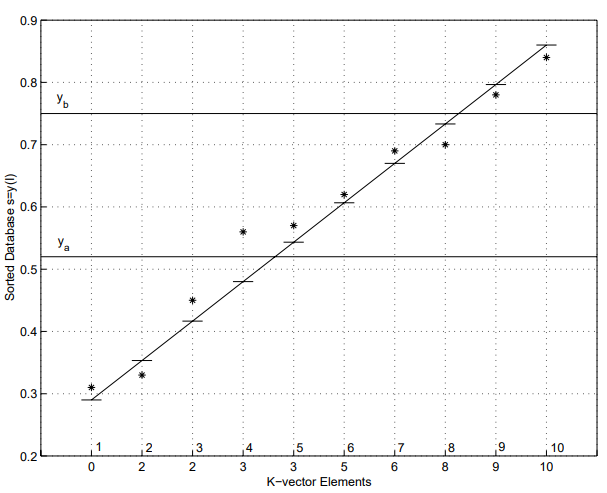
\includegraphics[width=0.5\textwidth]{images/k_vector.png}
	\caption{Exemplo da construção de um K vector. Fonte: ~\cite[]{Mortari}}
	\label{fig:K_vector} 
\end{figure}

No caso apresentado na figura ~\ref{fig:K_vector}, vemos que os dados se comportam de forma linear, e portanto podemos criar um modelo matemático para a relação entre o index do banco de dados e o valor do dado associado, utilizando uma relação linear obtida através do método dos minimos quadrados pelas equações ~\ref{eq:Beta_linear}, ~\ref{eq:Alpha_linear} e ~\ref{eq:Regressao_linear}.

\begin{equation}
	\beta = \frac{\sum_{i=1}^{n} (x_i - \bar{x})(y_i - \bar{y})}{\sum_{i=1}^{n} (x_i - \bar{x})^2}
	\label{eq:Beta_linear}
\end{equation}

\begin{equation}
	\alpha = \bar{y} - \beta * \bar{x}
	\label{eq:Alpha_linear}
\end{equation}

\begin{equation}
	y = \alpha + \beta * x
	\label{eq:Regressao_linear}
\end{equation}

Método de regressão retorna uma equação resposta com um erro associado, nesta aplicação pode-se testar o erro para cada ponto do banco de dados e averiguar o maior erro possível.
Dessa forma se obtém uma fórmula que diz qual o menor e o maior index possível em que uma metida posssa estar.

Se houver um vetor de tamanho \textbf{n}, com todas os valores conhecidos podemos reduzir o tempo de pesquisa que normalmente é de O(n*log(n)) para O(2*error*log(2*error)), 
diminuí-se o tamanho do vetor de pesquisa a 2 vezes o erro máximo da linearização, dessa forma os algorítimos de busca binária só precisam executar a pesquisa neste vetor selecionado.

\subsubsection{Quad Tree}

\subsubsection{Lost particle problem}
